\nonstopmode


\documentclass[a4paper,12pt,twoside,headings=small,bibliography=totocnumbered,headsepline]{scrartcl}
\RequirePackage{ifthen}




\usepackage{graphicx}


\usepackage{times}
\usepackage[T1]{fontenc} 
\usepackage[english]{babel}
\usepackage{color}


\usepackage{rotating}
\usepackage{lscape}


\usepackage[square, numbers, super]{natbib}


\usepackage{url}


\usepackage{tabularx}
\usepackage{array}
\usepackage{ctable}


\usepackage{listings}
\usepackage{fancyvrb}
\definecolor{lightgrey}{rgb}{0.95,0.95,0.95}


\pagestyle{headings}


\frenchspacing


\usepackage{setspace}


\pdfpagebox 4


\usepackage[printonlyused,withpage,footnote]{acronym}


\makeatletter
\lst@AddToHook{TextStyle}{\let\lst@basicstyle\ttfamily\small\fontfamily{pcr}\selectfont}
\makeatother



%
\newenvironment{numcodestyle}{
	\lstset{basicstyle=\footnotesize, numbers=left, numberstyle=\tiny, numbersep=3mm, stepnumber=1, backgroundcolor=\color{lightgrey}}
} 



%
\newenvironment{codetiny}{
	\lstset{basicstyle=\tiny, numbers=none, backgroundcolor=\color{lightgrey}}
} 



%
\newenvironment{codefoot}{
	\lstset{basicstyle=\footnotesize, numbers=none, backgroundcolor=\color{lightgrey}}
} 



%
\newenvironment{codescript}{
	\lstset{basicstyle=\scriptsize, numbers=none, backgroundcolor=\color{lightgrey}}
} 



%
\newenvironment{mydesc}{
	\begin{description}
	  \setlength{\itemsep}{1pt}
	  \setlength{\parskip}{0pt}
	  \setlength{\parsep}{0pt}
}
{
	\end{description}
} 



%
\newenvironment{condensed_enum}{
	\begin{enumerate}
	  \setlength{\itemsep}{1pt}
	  \setlength{\parskip}{0pt}
	  \setlength{\parsep}{0pt}
}
{
	\end{enumerate}
} 



%
\newenvironment{condensed_item}{
	\begin{itemize}
      \renewcommand{\labelitemi}{$\circ$}
	  \setlength{\itemsep}{1pt}
	  \setlength{\parskip}{0pt}
	  \setlength{\parsep}{0pt}
}
{
	\end{itemize}
} 


\newcolumntype{+}{>{\global\let\currentrowstyle\relax}}
\newcolumntype{^}{>{\currentrowstyle}}%
\providecommand{\rowstyle}[1]{\gdef \currentrowstyle{#1}%
#1\ignorespaces
} 





\pagecolor[gray]{.7}

\usepackage[latin1]{inputenc}



\makeatletter

\makeatletter
\count@=\the\catcode`\_ \catcode`\_=8 
\newenvironment{tex2html_wrap}{}{}%
\catcode`\<=12\catcode`\_=\count@
\newcommand{\providedcommand}[1]{\expandafter\providecommand\csname #1\endcsname}%
\newcommand{\renewedcommand}[1]{\expandafter\providecommand\csname #1\endcsname{}%
  \expandafter\renewcommand\csname #1\endcsname}%
\newcommand{\newedenvironment}[1]{\newenvironment{#1}{}{}\renewenvironment{#1}}%
\let\newedcommand\renewedcommand
\let\renewedenvironment\newedenvironment
\makeatother
\let\mathon=$
\let\mathoff=$
\ifx\AtBeginDocument\undefined \newcommand{\AtBeginDocument}[1]{}\fi
\newbox\sizebox
\setlength{\hoffset}{0pt}\setlength{\voffset}{0pt}
\addtolength{\textheight}{\footskip}\setlength{\footskip}{0pt}
\addtolength{\textheight}{\topmargin}\setlength{\topmargin}{0pt}
\addtolength{\textheight}{\headheight}\setlength{\headheight}{0pt}
\addtolength{\textheight}{\headsep}\setlength{\headsep}{0pt}
\setlength{\textwidth}{349pt}
\newwrite\lthtmlwrite
\makeatletter
\let\realnormalsize=\normalsize
\global\topskip=2sp
\def\preveqno{}\let\real@float=\@float \let\realend@float=\end@float
\def\@float{\let\@savefreelist\@freelist\real@float}
\def\liih@math{\ifmmode$\else\bad@math\fi}
\def\end@float{\realend@float\global\let\@freelist\@savefreelist}
\let\real@dbflt=\@dbflt \let\end@dblfloat=\end@float
\let\@largefloatcheck=\relax
\let\if@boxedmulticols=\iftrue
\def\@dbflt{\let\@savefreelist\@freelist\real@dbflt}
\def\adjustnormalsize{\def\normalsize{\mathsurround=0pt \realnormalsize
 \parindent=0pt\abovedisplayskip=0pt\belowdisplayskip=0pt}%
 \def\phantompar{\csname par\endcsname}\normalsize}%
\def\lthtmltypeout#1{{\let\protect\string \immediate\write\lthtmlwrite{#1}}}%
\newcommand\lthtmlhboxmathA{\adjustnormalsize\setbox\sizebox=\hbox\bgroup\kern.05em }%
\newcommand\lthtmlhboxmathB{\adjustnormalsize\setbox\sizebox=\hbox to\hsize\bgroup\hfill }%
\newcommand\lthtmlvboxmathA{\adjustnormalsize\setbox\sizebox=\vbox\bgroup %
 \let\ifinner=\iffalse \let\)\liih@math }%
\newcommand\lthtmlboxmathZ{\@next\next\@currlist{}{\def\next{\voidb@x}}%
 \expandafter\box\next\egroup}%
\newcommand\lthtmlmathtype[1]{\gdef\lthtmlmathenv{#1}}%
\newcommand\lthtmllogmath{\dimen0\ht\sizebox \advance\dimen0\dp\sizebox
  \ifdim\dimen0>.95\vsize
   \lthtmltypeout{%
*** image for \lthtmlmathenv\space is too tall at \the\dimen0, reducing to .95 vsize ***}%
   \ht\sizebox.95\vsize \dp\sizebox\z@ \fi
  \lthtmltypeout{l2hSize %
:\lthtmlmathenv:\the\ht\sizebox::\the\dp\sizebox::\the\wd\sizebox.\preveqno}}%
\newcommand\lthtmlfigureA[1]{\let\@savefreelist\@freelist
       \lthtmlmathtype{#1}\lthtmlvboxmathA}%
\newcommand\lthtmlpictureA{\bgroup\catcode`\_=8 \lthtmlpictureB}%
\newcommand\lthtmlpictureB[1]{\lthtmlmathtype{#1}\egroup
       \let\@savefreelist\@freelist \lthtmlhboxmathB}%
\newcommand\lthtmlpictureZ[1]{\hfill\lthtmlfigureZ}%
\newcommand\lthtmlfigureZ{\lthtmlboxmathZ\lthtmllogmath\copy\sizebox
       \global\let\@freelist\@savefreelist}%
\newcommand\lthtmldisplayA{\bgroup\catcode`\_=8 \lthtmldisplayAi}%
\newcommand\lthtmldisplayAi[1]{\lthtmlmathtype{#1}\egroup\lthtmlvboxmathA}%
\newcommand\lthtmldisplayB[1]{\edef\preveqno{(\theequation)}%
  \lthtmldisplayA{#1}\let\@eqnnum\relax}%
\newcommand\lthtmldisplayZ{\lthtmlboxmathZ\lthtmllogmath\lthtmlsetmath}%
\newcommand\lthtmlinlinemathA{\bgroup\catcode`\_=8 \lthtmlinlinemathB}
\newcommand\lthtmlinlinemathB[1]{\lthtmlmathtype{#1}\egroup\lthtmlhboxmathA
  \vrule height1.5ex width0pt }%
\newcommand\lthtmlinlineA{\bgroup\catcode`\_=8 \lthtmlinlineB}%
\newcommand\lthtmlinlineB[1]{\lthtmlmathtype{#1}\egroup\lthtmlhboxmathA}%
\newcommand\lthtmlinlineZ{\egroup\expandafter\ifdim\dp\sizebox>0pt %
  \expandafter\centerinlinemath\fi\lthtmllogmath\lthtmlsetinline}
\newcommand\lthtmlinlinemathZ{\egroup\expandafter\ifdim\dp\sizebox>0pt %
  \expandafter\centerinlinemath\fi\lthtmllogmath\lthtmlsetmath}
\newcommand\lthtmlindisplaymathZ{\egroup %
  \centerinlinemath\lthtmllogmath\lthtmlsetmath}
\def\lthtmlsetinline{\hbox{\vrule width.1em \vtop{\vbox{%
  \kern.1em\copy\sizebox}\ifdim\dp\sizebox>0pt\kern.1em\else\kern.3pt\fi
  \ifdim\hsize>\wd\sizebox \hrule depth1pt\fi}}}
\def\lthtmlsetmath{\hbox{\vrule width.1em\kern-.05em\vtop{\vbox{%
  \kern.1em\kern0.8 pt\hbox{\hglue.17em\copy\sizebox\hglue0.8 pt}}\kern.3pt%
  \ifdim\dp\sizebox>0pt\kern.1em\fi \kern0.8 pt%
  \ifdim\hsize>\wd\sizebox \hrule depth1pt\fi}}}
\def\centerinlinemath{%
  \dimen1=\ifdim\ht\sizebox<\dp\sizebox \dp\sizebox\else\ht\sizebox\fi
  \advance\dimen1by.5pt \vrule width0pt height\dimen1 depth\dimen1 
 \dp\sizebox=\dimen1\ht\sizebox=\dimen1\relax}

\def\lthtmlcheckvsize{\ifdim\ht\sizebox<\vsize 
  \ifdim\wd\sizebox<\hsize\expandafter\hfill\fi \expandafter\vfill
  \else\expandafter\vss\fi}%
\providecommand{\selectlanguage}[1]{}%
\makeatletter \tracingstats = 1 


\begin{document}
\pagestyle{empty}\thispagestyle{empty}\lthtmltypeout{}%
\lthtmltypeout{latex2htmlLength hsize=\the\hsize}\lthtmltypeout{}%
\lthtmltypeout{latex2htmlLength vsize=\the\vsize}\lthtmltypeout{}%
\lthtmltypeout{latex2htmlLength hoffset=\the\hoffset}\lthtmltypeout{}%
\lthtmltypeout{latex2htmlLength voffset=\the\voffset}\lthtmltypeout{}%
\lthtmltypeout{latex2htmlLength topmargin=\the\topmargin}\lthtmltypeout{}%
\lthtmltypeout{latex2htmlLength topskip=\the\topskip}\lthtmltypeout{}%
\lthtmltypeout{latex2htmlLength headheight=\the\headheight}\lthtmltypeout{}%
\lthtmltypeout{latex2htmlLength headsep=\the\headsep}\lthtmltypeout{}%
\lthtmltypeout{latex2htmlLength parskip=\the\parskip}\lthtmltypeout{}%
\lthtmltypeout{latex2htmlLength oddsidemargin=\the\oddsidemargin}\lthtmltypeout{}%
\makeatletter
\if@twoside\lthtmltypeout{latex2htmlLength evensidemargin=\the\evensidemargin}%
\else\lthtmltypeout{latex2htmlLength evensidemargin=\the\oddsidemargin}\fi%
\lthtmltypeout{}%
\makeatother
\setcounter{page}{1}
\onecolumn

% !!! IMAGES START HERE !!!



\selectlanguage{english}

\stepcounter{section}
\stepcounter{subsection}
\stepcounter{subsection}
\stepcounter{subsubsection}
\stepcounter{subsubsection}
\stepcounter{section}
\stepcounter{subsection}
{\newpage\clearpage
% contents=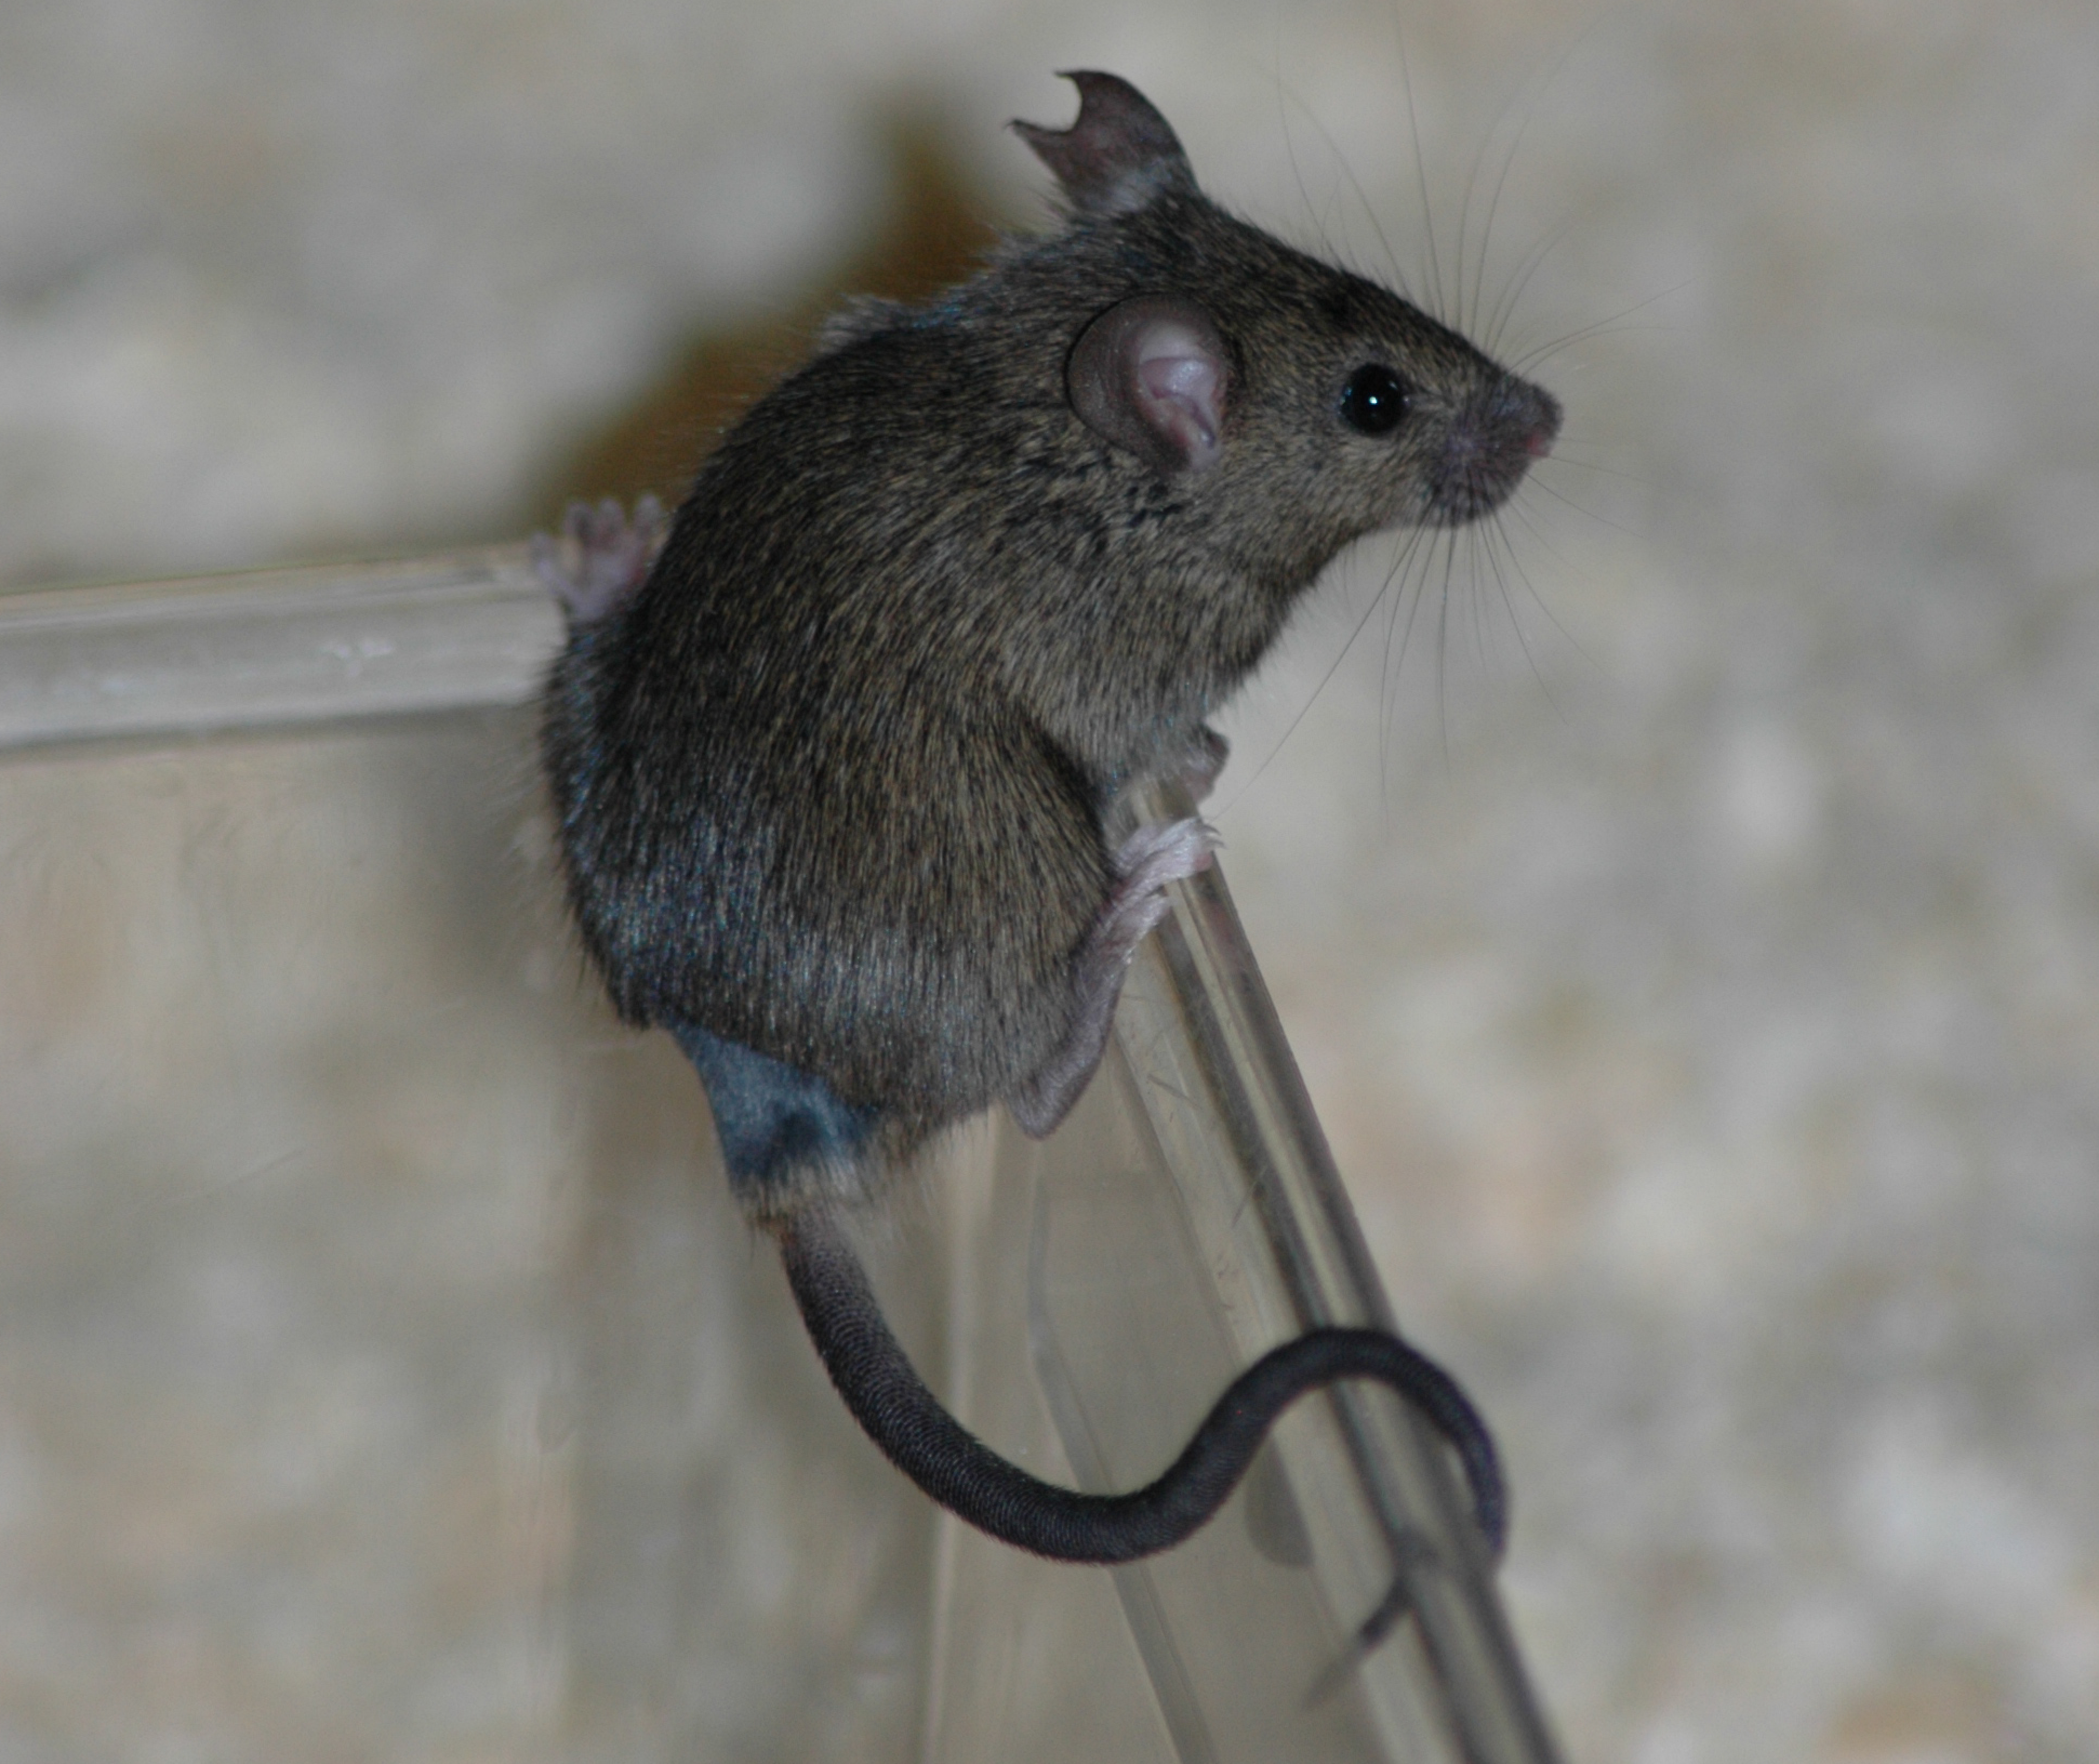
\includegraphics[width=0.5\textwidth]{assets/pdf/mus_domesticus.pdf}
\lthtmlpictureA{tex2html_wrap1156}%
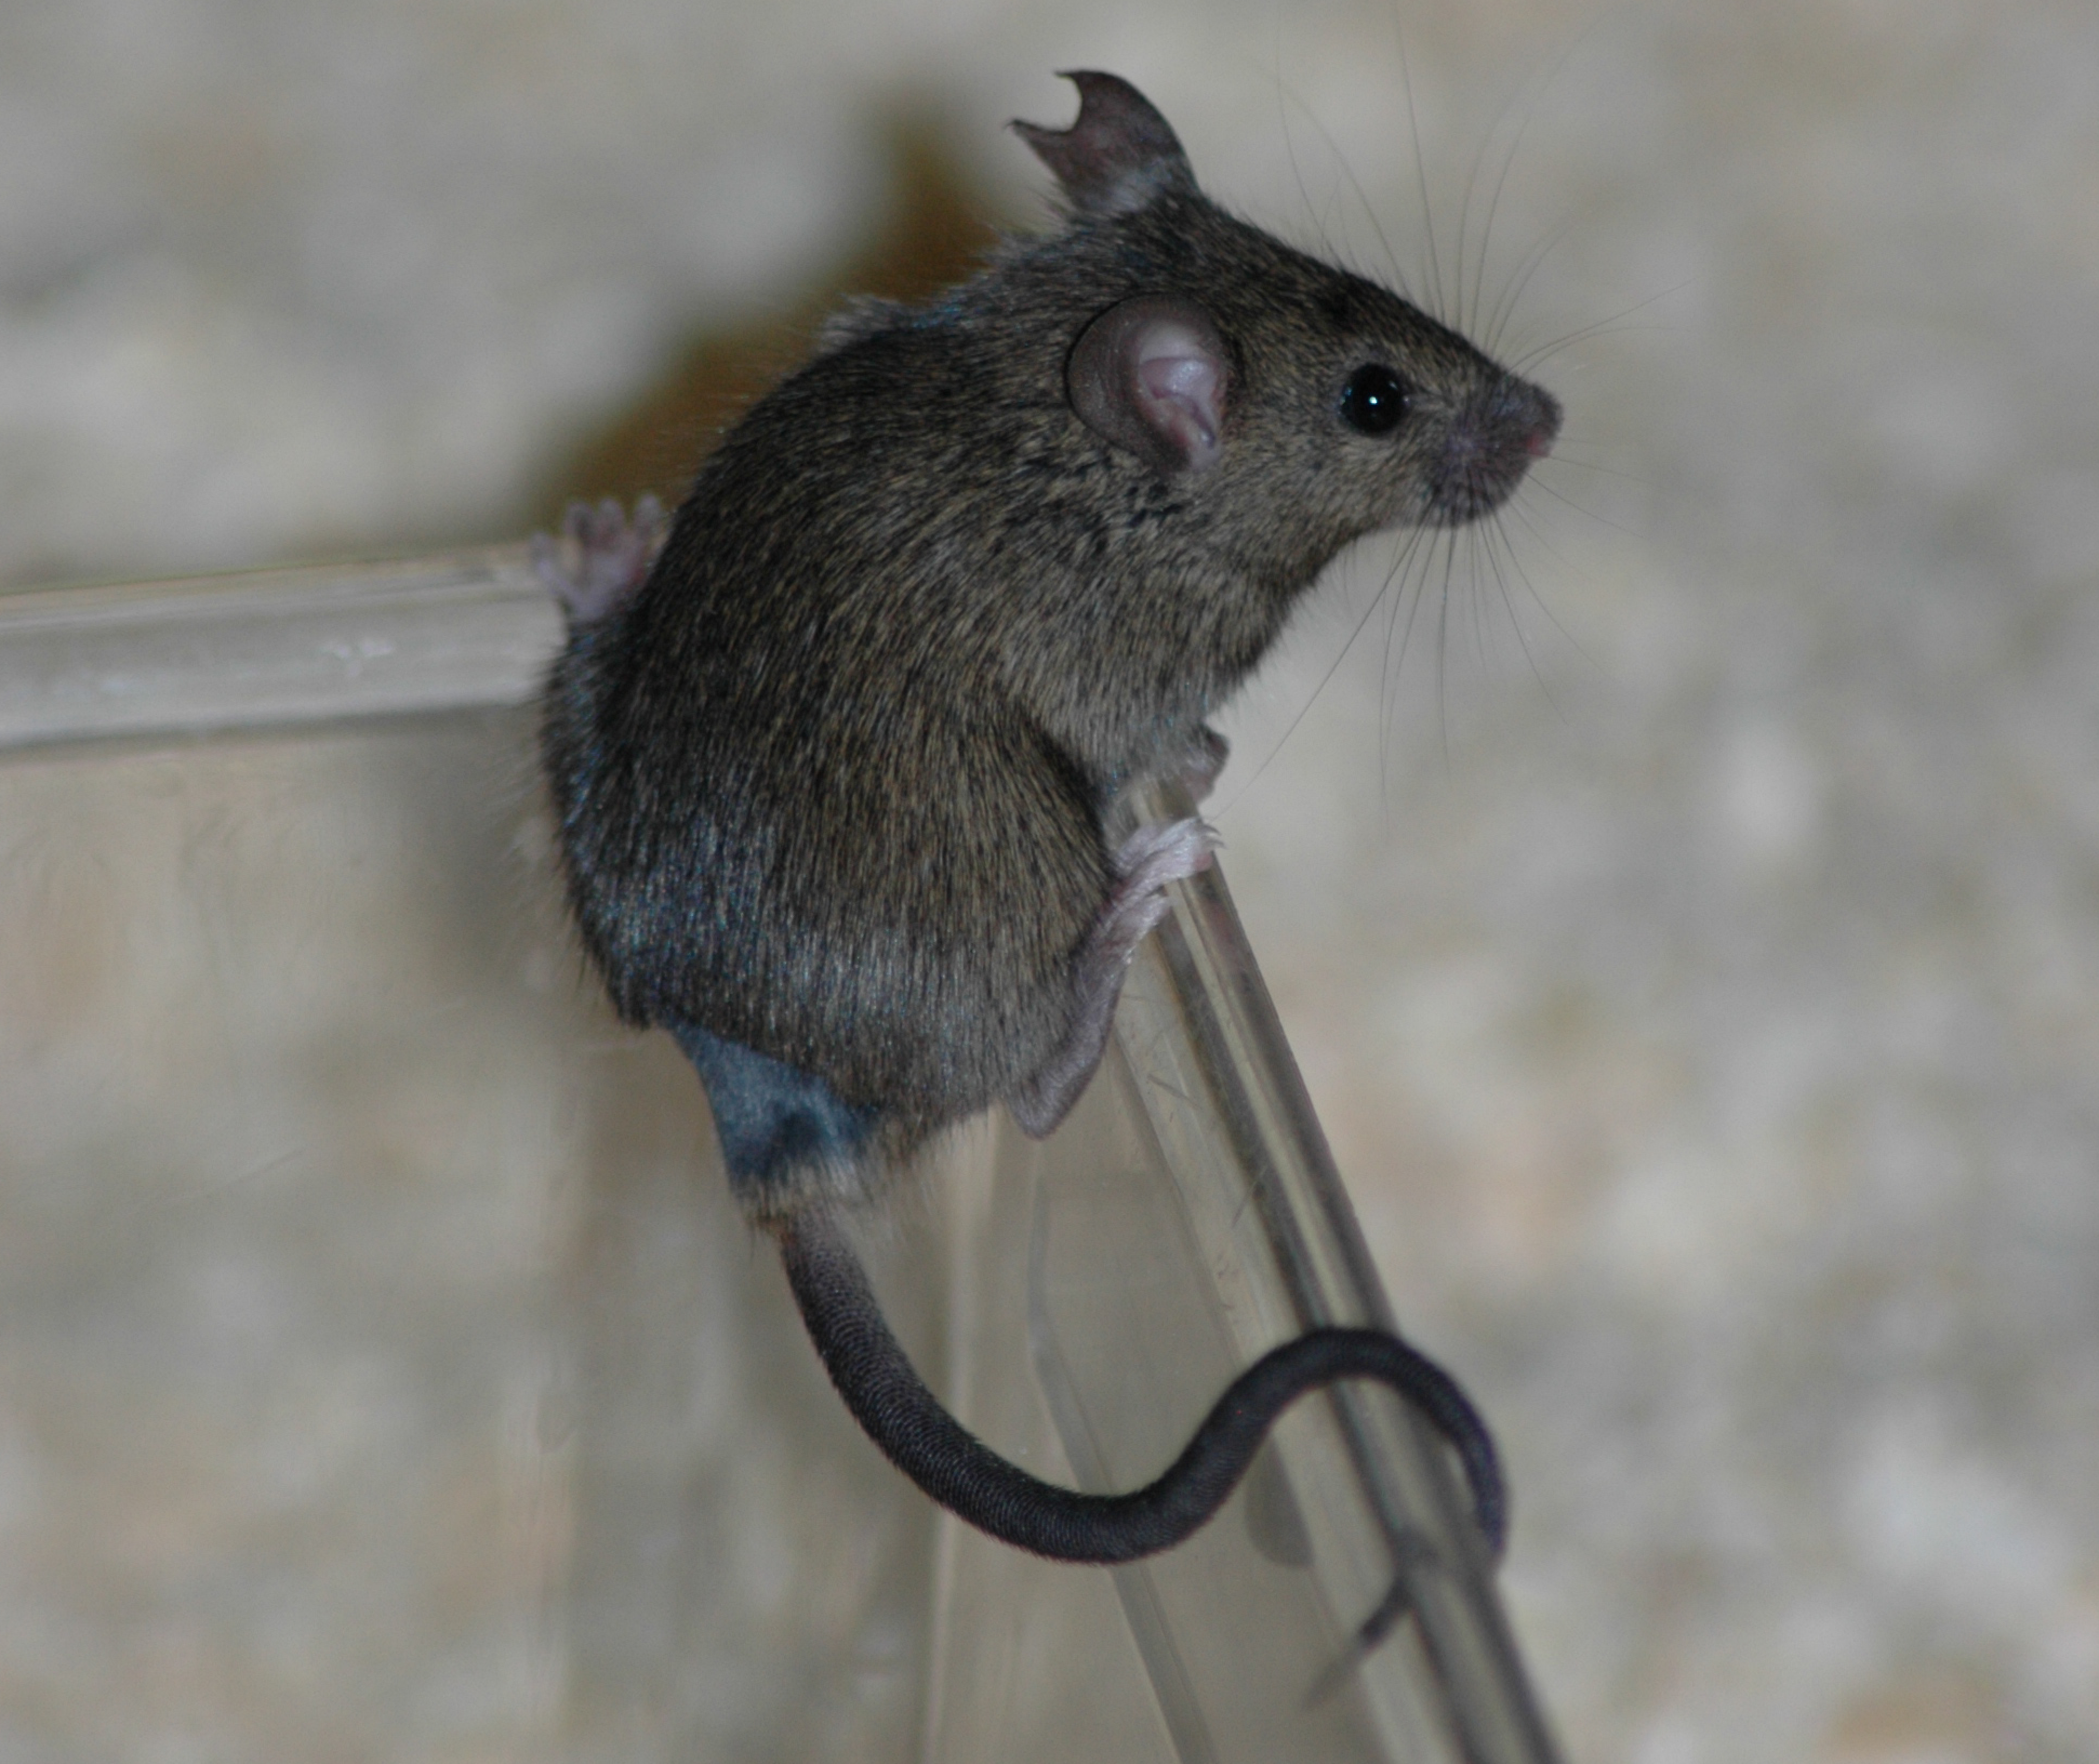
\includegraphics[width=0.5\textwidth]{assets/pdf/mus_domesticus.pdf}%
\lthtmlpictureZ
\lthtmlcheckvsize\clearpage}

\stepcounter{subsection}
\stepcounter{subsection}
\stepcounter{subsubsection}
\stepcounter{subsubsection}
\stepcounter{section}
{\newpage\clearpage
% contents=$^2$
\lthtmlinlinemathA{tex2html_wrap_inline352}%
$^2$%
\lthtmlinlinemathZ
\lthtmlcheckvsize\clearpage}

{\newpage\clearpage
% contents=\includegraphics[width=0.5\textwidth]{assets/pdf/shed_overview.pdf}
\lthtmlpictureA{tex2html_wrap1166}%
\includegraphics[width=0.5\textwidth]{assets/pdf/shed_overview.pdf}%
\lthtmlpictureZ
\lthtmlcheckvsize\clearpage}

{\newpage\clearpage
% contents=\includegraphics[width=\textwidth]{assets/pdf/shed_schema.pdf}
\lthtmlpictureA{tex2html_wrap1170}%
\includegraphics[width=\textwidth]{assets/pdf/shed_schema.pdf}%
\lthtmlpictureZ
\lthtmlcheckvsize\clearpage}

\stepcounter{section}
{\newpage\clearpage
% contents=\includegraphics[width=0.5\textwidth]{assets/pdf/transponder_inject.pdf}
\lthtmlpictureA{tex2html_wrap1175}%
\includegraphics[width=0.5\textwidth]{assets/pdf/transponder_inject.pdf}%
\lthtmlpictureZ
\lthtmlcheckvsize\clearpage}

\stepcounter{subsection}
{\newpage\clearpage
% contents=\includegraphics[width=\textwidth]{assets/pdf/box_schema.pdf}
\lthtmlpictureA{tex2html_wrap1180}%
\includegraphics[width=\textwidth]{assets/pdf/box_schema.pdf}%
\lthtmlpictureZ
\lthtmlcheckvsize\clearpage}

\stepcounter{subsubsection}
{\newpage\clearpage
% contents=\includegraphics[width=0.8\textwidth]{assets/pdf/dataset.pdf}
\lthtmlpictureA{tex2html_wrap1185}%
\includegraphics[width=0.8\textwidth]{assets/pdf/dataset.pdf}%
\lthtmlpictureZ
\lthtmlcheckvsize\clearpage}

{\newpage\clearpage
% contents=\includegraphics[width=0.8\textwidth]{assets/pdf/dataset_no_data.pdf}
\lthtmlpictureA{tex2html_wrap1189}%
\includegraphics[width=0.8\textwidth]{assets/pdf/dataset_no_data.pdf}%
\lthtmlpictureZ
\lthtmlcheckvsize\clearpage}

{\newpage\clearpage
% contents=begin{lstlisting}[frame=none] 2008-10-01 16:31:08:499;   111;   0;  2008-10-01 16:31:09:095;   113;   0;  2008-10-01 16:31:42:512;   111;   5;  00 06 B8 D4 5A 2008-10-01 16:31:42:807;   113;   5;  00...}
\lthtmlfigureA{lstlisting426}%
\begin{lstlisting}[frame=none]
2008-10-01 16:31:08:499;   111;   0; 
2008-10-01 16:31:09:095;   113;   0; 
2008-10-01 16:31:42:512;   111;   5;  00 06 B8 D4 5A
2008-10-01 16:31:42:807;   113;   5;  00 06 B8 D4 5A
2008-10-01 16:31:43:619;   111;   0; 
2008-10-01 16:31:44:014;   113;   0;
\end{lstlisting}%
\lthtmlfigureZ
\lthtmlcheckvsize\clearpage}



\setlength{\itemsep}{1pt}%

\setlength{\itemsep}{1pt}


\setlength{\parskip}{0pt}%

\setlength{\parskip}{0pt}


\setlength{\parsep}{0pt}%

\setlength{\parsep}{0pt}
\stepcounter{subsubsection}
\stepcounter{subsubsection}
\stepcounter{subsubsection}
\stepcounter{subsection}
\stepcounter{subsection}
{\newpage\clearpage
% contents=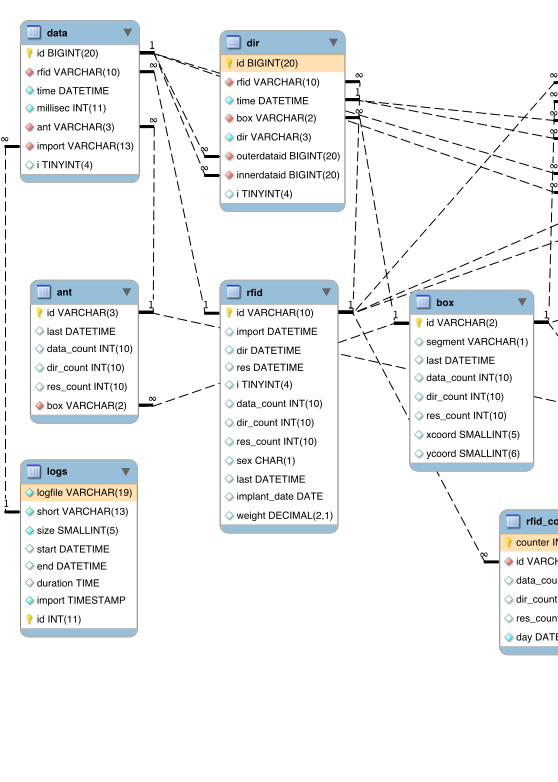
\includegraphics[width=\textwidth]{assets/pdf/micedata_schema.pdf}
\lthtmlpictureA{tex2html_wrap1198}%
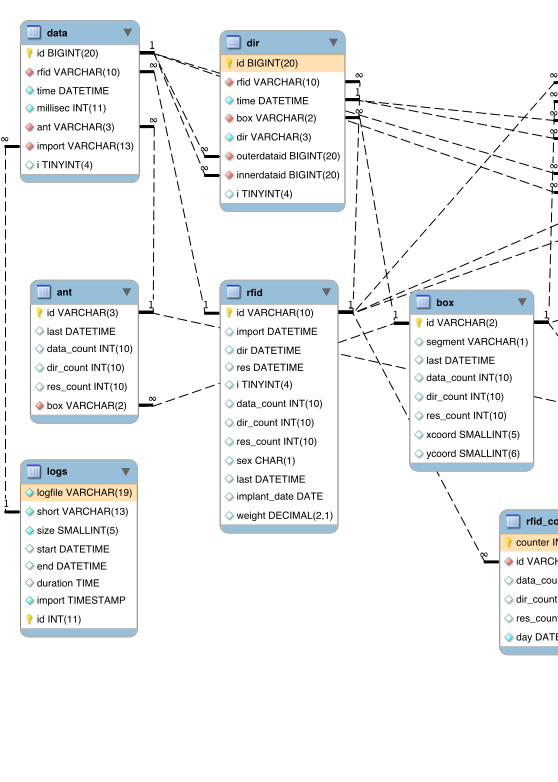
\includegraphics[width=\textwidth]{assets/pdf/micedata_schema.pdf}%
\lthtmlpictureZ
\lthtmlcheckvsize\clearpage}

\stepcounter{subsubsection}
{\newpage\clearpage
% contents=\includegraphics[width=\textwidth]{assets/pdf/processed_data_schema.pdf}
\lthtmlpictureA{tex2html_wrap1203}%
\includegraphics[width=\textwidth]{assets/pdf/processed_data_schema.pdf}%
\lthtmlpictureZ
\lthtmlcheckvsize\clearpage}

\stepcounter{paragraph}
{\newpage\clearpage
% contents=begin{lstlisting}[frame=none] +---------+------------+---------------------+----------+-----+---------------+------+ | id      | rfid       | time                | millisec | ant | import        | i ...}
\lthtmlfigureA{lstlisting498}%
\begin{lstlisting}[frame=none]
+---------+------------+---------------------+----------+-----+---------------+------+
| id      | rfid       | time                | millisec | ant | import        | i    |
+---------+------------+---------------------+----------+-----+---------------+------+
| 8184253 | 0006CD3416 | 2009-03-27 17:07:40 |       71 | 113 | 09-0326170750 |    2 | 
+---------+------------+---------------------+----------+-----+---------------+------+
\end{lstlisting}%
\lthtmlfigureZ
\lthtmlcheckvsize\clearpage}



\setlength{\itemsep}{1pt}%

\setlength{\itemsep}{1pt}


\setlength{\parskip}{0pt}%

\setlength{\parskip}{0pt}


\setlength{\parsep}{0pt}%

\setlength{\parsep}{0pt}
\stepcounter{paragraph}
{\newpage\clearpage
% contents=begin{lstlisting}[frame=none] +---------+------------+---------------------+-----+-----+-------------+-------------+------+ | id      | rfid       | time                | box | dir | outerdataid | in...}
\lthtmlfigureA{lstlisting517}%
\begin{lstlisting}[frame=none]
+---------+------------+---------------------+-----+-----+-------------+-------------+------+
| id      | rfid       | time                | box | dir | outerdataid | innerdataid | i    |
+---------+------------+---------------------+-----+-----+-------------+-------------+------+
| 2721669 | 0006CD3416 | 2009-03-27 17:07:40 | 11  | in  |     8184252 |     8184253 |    1 | 
+---------+------------+---------------------+-----+-----+-------------+-------------+------+
\end{lstlisting}%
\lthtmlfigureZ
\lthtmlcheckvsize\clearpage}



\setlength{\itemsep}{1pt}%

\setlength{\itemsep}{1pt}


\setlength{\parskip}{0pt}%

\setlength{\parskip}{0pt}


\setlength{\parsep}{0pt}%

\setlength{\parsep}{0pt}
\stepcounter{paragraph}
{\newpage\clearpage
% contents=begin{lstlisting}[frame=none] ++--------+------------+-----+---------------------+---------------------+----------+---------+---------+------+----------+ | id     | rfid       | box | box_in         ...}
\lthtmlfigureA{lstlisting538}%
\begin{lstlisting}[frame=none]
++--------+------------+-----+---------------------+---------------------+----------+---------+---------+------+----------+
| id     | rfid       | box | box_in              | box_out             | dt       | inid    | outid   | i    | meetings |
+--------+------------+-----+---------------------+---------------------+----------+---------+---------+------+----------+
| 593660 | 0006CC7646 | 28  | 2009-03-27 13:48:34 | 2009-03-27 17:05:56 | 03:17:22 | 2872164 | 8184246 |    4 | TRUE     | 
+--------+------------+-----+---------------------+---------------------+----------+---------+---------+------+----------+
\par
\end{lstlisting}%
\lthtmlfigureZ
\lthtmlcheckvsize\clearpage}



\setlength{\itemsep}{1pt}%

\setlength{\itemsep}{1pt}


\setlength{\parskip}{0pt}%

\setlength{\parskip}{0pt}


\setlength{\parsep}{0pt}%

\setlength{\parsep}{0pt}
\stepcounter{paragraph}
\stepcounter{subsubsection}
\stepcounter{paragraph}
\stepcounter{paragraph}
\stepcounter{paragraph}
\stepcounter{subsubsection}
\stepcounter{paragraph}
\stepcounter{subsection}
\stepcounter{section}
\stepcounter{subsection}
\stepcounter{subsection}
\stepcounter{subsection}
\stepcounter{subsection}
\stepcounter{section}
\stepcounter{subsection}
\stepcounter{subsubsection}
\stepcounter{subsubsection}
\stepcounter{subsubsection}
\stepcounter{subsection}
\stepcounter{subsubsection}
\stepcounter{paragraph}
\stepcounter{subsubsection}
\stepcounter{paragraph}
\stepcounter{subsubsection}
\stepcounter{paragraph}
\stepcounter{subsubsection}
\stepcounter{paragraph}
\stepcounter{section}
\stepcounter{subsection}
\stepcounter{subsection}
\stepcounter{subsection}
\stepcounter{subsection}
\stepcounter{subsubsection}
\stepcounter{subsubsection}
\stepcounter{subsubsection}
\stepcounter{subsection}
\stepcounter{subsubsection}
\stepcounter{subsubsection}
\stepcounter{subsubsection}
\stepcounter{subsubsection}
\stepcounter{subsubsection}
\stepcounter{subsubsection}
\stepcounter{subsubsection}
\stepcounter{paragraph}
\stepcounter{section}
\stepcounter{section}
\stepcounter{subsection}
\stepcounter{subsubsection}
\stepcounter{section}
{\newpage\clearpage
% contents=\includegraphics[width=\textwidth]{assets/pdf/app_design.pdf}
\lthtmlpictureA{tex2html_wrap1260}%
\includegraphics[width=\textwidth]{assets/pdf/app_design.pdf}%
\lthtmlpictureZ
\lthtmlcheckvsize\clearpage}

{\newpage\clearpage
% contents=begin{sidewaystable} % latex2html id marker 1039  \caption{Meaning of the i values in the data tables.} begin{tabularx}{\textheight}{>{\bfseries }+lp{2cm}^X^X^X^X^X} \toprule \gdef \currentrowstyle{...}
\lthtmlfigureA{sidewaystable1039}%
\begin{sidewaystable}
% latex2html id marker 1039

\caption{Meaning of the i values in the data tables.}
\begin{tabularx}{\textheight}{>{\bfseries }+lp{2cm}^X^X^X^X^X}
\toprule
\gdef \currentrowstyle{\bfseries }\bfseries\ignorespaces 
&	0	&	1	&	2	&	3	&	4\\\hline
data	    &  Dataset has not analyzed yet.  &  Dataset has been analyzed but no matching dataset to form a direction result could be found.	&	Dataset is part of a direction result (either a value in column \lstinline|innerdataid| or column \lstinline|outerdataid| of a dataset in the \lstinline|dir| table).	&	Dataset is part of a typ 3 result.	&	Dataset is part of a typ 4 result.\\\midrule
\par
dir     	& AveC & Average cost across all genomes in population\\\midrule
\par
res     	& AveF & Average fitness of all genomes\\\midrule
\par
meetings    & MinC & The lowest cost from any genome (ignoring overfill)\\\bottomrule
\end{tabularx}
\par
\end{sidewaystable}%
\lthtmlfigureZ
\lthtmlcheckvsize\clearpage}

{\newpage\clearpage
% contents=begin{sidewaysfigure} % latex2html id marker 1049    \includegraphics[width=\textwidth]{assets/pdf/micedata_data_processing_cheatsheet.pdf}   \caption[Data processing cheatsheet]{Cheatsheet for the d...}
\lthtmlfigureA{sidewaysfigure1049}%
\begin{sidewaysfigure}
% latex2html id marker 1049

  \includegraphics[width=\textwidth]{assets/pdf/micedata_data_processing_cheatsheet.pdf}
  \caption[Data processing cheatsheet]{Cheatsheet for the data processing steps.}
  
\end{sidewaysfigure}%
\lthtmlfigureZ
\lthtmlcheckvsize\clearpage}

\stepcounter{section}
{\newpage\clearpage
% contents=begin{acronym} \acro{RDBMS}[Relational Database Management System]{A Relational Database Management System is a \acs{DBMS} in which data is stored in the form of tables and the relationship among the...}
\lthtmlfigureA{acronym1055}%
\begin{acronym}
\acro{RDBMS}[Relational Database Management System]{A Relational Database Management System is a \acs{DBMS} in which data is stored in the form of tables and the relationship among the data is also stored in the form of tables. \cite{wiki:rdms}}
\acro{DBMS}[Database Management System]{A Database Management System is computer software that manages databases. \cite{wiki:dbms}}
\acro{RFID}[Radio-frequency identification]{Radio-frequency identification (RFID) is the use of an object (typically referred to as an RFID tag) applied to or incorporated into a product, animal, or person for the purpose of identification and tracking using radio waves.\cite{wiki:rfid} }
\acro{SQL}[Structured Query Language]{The Structured Query Language is a database computer language designed for the retrieval and management of data in relational database management systems.\cite{wiki:sql}}
\acro{KJ}[KJ]{The Joule is a derived unit of energy and defined as the work done by a force of one newton travelling through a distance of one metre. \cite{wiki:joule}. 1 Kilo Joule = 10$^3$\  Joule.}
\acro{perl}[perl]{Perl is a high-level, general-purpose, interpreted, dynamic programming language. \cite{wiki:perl}}
\end{acronym}%
\lthtmlfigureZ
\lthtmlcheckvsize\clearpage}


\end{document}
